\section{Plan: domains, money, team and risks}\label{sec:plan}

\evfut{} Everything in this section is future work, and every figure is a planning range.

\subsection{Domains}

A domain is chosen for the generalization question it answers and the human criterion that can test it,
never for convenient data (\cref{tab:domains}). Three binding rules apply. Physics is the frozen Track~A
domain and enters only through sealed predictions. A held-out gold domain is never reconstructed before
its configuration is frozen: its first reconstruction \emph{is} the test run. PLC and GDPR tuned the
lexicons, so they never carry a gate reading. Hence the recommended design: a V5 pilot in PLC, not
analyzed for effect, and the V5 main study in a fresh maintenance-diagnosis task (D3) and a held-out
regulation (D4).

\begin{table}[htbp]
  \centering\footnotesize
  \caption{The six proposed domains. D1, D3 and D4 carry H2's gates; D2 carries H-OSS only; D5 and D6
    gate nothing for H2.}
  \label{tab:domains}
  \begin{tabularx}{\linewidth}{@{}>{\raggedright\arraybackslash}p{0.17\linewidth}
      >{\raggedright\arraybackslash}X>{\raggedright\arraybackslash}p{0.27\linewidth}
      >{\raggedright\arraybackslash}p{0.17\linewidth}@{}}
    \toprule
    Domain & Question & Criterion & Role \\
    \midrule
    D1 Clinical procedure & Does the map find omitted steps and cues in a decision-heavy procedure? &
      Pooled published CTA golds, Sullivan's 46-item list first & V2; MS3 screen \\
    D2 Open-source maintenance & Does artifact coverage predict realized knowledge loss? & Blind-coded
      trouble after truck-factor departures & V3 (H-OSS); V7 precursor \\
    D3 Industrial fault diagnosis & Does it hold where craft dominates and text is poor? & Prospective
      blind elicitation & V5; MS5 \\
    D4 Regulatory judgment & Does it work where the residual sits in hedges and exceptions? &
      Prospective blind elicitation & V5; MS5 \\
    D5 School mathematics & Does an expert-text residual relate to learner difficulty? & Public learner
      response data & Learner link only \\
    D6 Introductory mechanics & Best-case ceiling where residual, learner error and an RCT meet & Track~A's
      own registered rules & Secondary, non-gating \\
    \bottomrule
  \end{tabularx}
\end{table}

\subsection{Roadmap and the money each gate releases}

\Cref{fig:roadmap} shows the phases. Phase~0 runs alone and needs no grant, no participants and no new
software. Phase~1 builds nothing for Phase~2, so no Phase~2 spending runs ahead of MS3. \Cref{tab:money}
gives each tranche. Personnel is costed at EUR~6--10k per person-month, to be replaced by the host
institution's rate.

\begin{figure}[tbp]
  \centering
  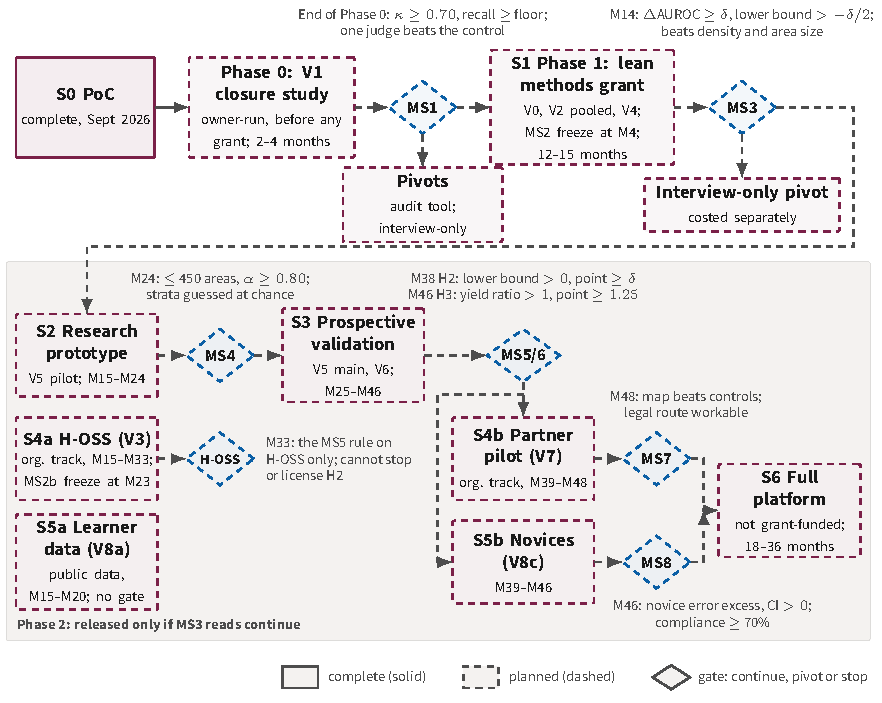
\includegraphics{figures/pdf/fig14_roadmap.pdf}
  \caption[Gated roadmap]{Which gated stages lead from PoC to platform? Phase~0 (owner-run, before any
    grant) is the closure study, ending at MS1. Phase~1, a lean methods grant, starts only on MS1
    CONTINUE and ends at the screening gate MS3. Phase~2 starts only on MS3 CONTINUE; its prospective
    study decides H2 at MS5. Every stop leads to a pivot with its own, smaller budget. Only S0, the PoC, is
    complete.}
  \label{fig:roadmap}
\end{figure}

\begin{table}[htbp]
  \centering\footnotesize
  \caption{Tranches, the gate that releases each, and indicative cost. Months count from the start of
    Phase~1.}
  \label{tab:money}
  \begin{tabularx}{\linewidth}{@{}>{\raggedright\arraybackslash}p{0.13\linewidth}
      >{\raggedright\arraybackslash}p{0.13\linewidth}>{\raggedright\arraybackslash}X
      >{\raggedright\arraybackslash}p{0.1\linewidth}r>{\raggedright\arraybackslash}p{0.13\linewidth}@{}}
    \toprule
    Tranche & Released by & Scope & Months & PM & Total (EUR) \\
    \midrule
    Phase~0 & Owner, no grant & V1 closure study & 2--4 mo before M1 & -- & $\approx 10^3$ \\
    Phase~1 & MS1 continue & Area score, freeze, V0, judge check, pooled V2, V4 & M1--M14 & 35--44 &
      \textbf{0.23--0.51\,M} \\
    2a & MS3 continue & Workbench, V5 pilot, learner data, ledger groundwork & M15--M24 & 29--44 &
      0.19--0.49\,M \\
    2b & MS4 continue & V5 main, powered & M25--M38 & 22--36 & 0.17--0.61\,M \\
    2c & MS5 continue & V6, V7, novice study, education pilot, on-prem stack & M39--M48 & 38--62 &
      0.26--0.79\,M \\
    O & MS3 continue & Git adapter, code lenses, V3 (H-OSS) & M15--M36 & 14--22 & 0.09--0.26\,M \\
    \midrule
    \textbf{Phase~2} & & 2a--2c and O & M15--M48 & 103--164 & \textbf{0.7--2.2\,M} \\
    \textbf{Program} & & Phases~1 and 2 & 48~mo & 138--208 & \textbf{0.9--2.7\,M} \\
    Interview-only pivot & MS1, MS3 or MS5 stop & Separate proposal & 18--24~mo & 21--31 & 0.14--0.38\,M
      \\
    \bottomrule
  \end{tabularx}
\end{table}

\evint{} \textbf{Money at risk if H2 fails}: at MS1, about EUR~$10^3$ plus the owner's time; at MS3,
Phase~1 (EUR~0.23--0.51\,M), which still leaves a released closure set, a frozen area score and a public
benchmark; at MS4, EUR~0.42--1.00\,M; at MS5, EUR~0.59--1.61\,M, and tranche 2c is never released. The
binding constraint of V5 is recruiting about 45 eligible experts, not money. \evobs{} The PoC's one hard
cost number: a reconstruction run cost \$0.50--\$1.00. Money was not the constraint; headroom was.
\evint{} So provider limits are set at least three times the sum of a stage's registered caps, the
headroom check runs as code, each experiment has its own key, and every study reports cost per
\emph{validated} item.

\subsection{Team}

\begin{evfutbox}
  \textbf{Team status.} No team exists yet: no host institution, no principal investigator (PI) record
  for this program, no statistician, no CTA collaborator, no gate reader and no letter of support. One
  operator designed, built, ran and read the PoC with AI assistance, and is the prospective applicant.
  Before MS1 is read: the non-owner blind coder and the external gate reader. Before the Phase~1
  proposal: host institution, PI, statistician as co-applicant, CTA collaborator, research engineer,
  data-protection and license advisor. Before Phase~2: a cognitive psychologist or CTA lead, expert
  pools with letters from professional bodies, and a learning scientist.
\end{evfutbox}

\evint{} The hard problems span language processing and measurement, CTA, learning science, statistics,
and security, privacy and law, so the team is interdisciplinary. It grows only when a gate releases the
next phase (\cref{tab:team}).

\begin{table}[htbp]
  \centering\footnotesize
  \caption{Team by phase. Phase~1 (12--15 months, about 2.5--3.0~FTE, 35--44 person-months) reaches
    MS3; Phase~2 (34 months, about 3.0--4.8~FTE on average across 6--8 people) is hired only on MS3
    CONTINUE. Full role tables: Extended Technical Report, Section~24 and Appendix~H.}
  \label{tab:team}
  \begin{tabularx}{\linewidth}{@{}>{\raggedright\arraybackslash}p{0.3\linewidth}
      >{\raggedright\arraybackslash}p{0.14\linewidth}>{\raggedright\arraybackslash}p{0.14\linewidth}
      >{\raggedright\arraybackslash}X@{}}
    \toprule
    Role & Phase~1 FTE & Phase~2 FTE & Main work \\
    \midrule
    PI / research lead & 0.8--1.0 & 0.5--1.0 & Hypotheses, thresholds, gate reports (never reads a
      gate) \\
    Research engineer (LLM / retrieval) & 1.0 & 0.5--1.0 & Area score, freeze, dated corpora; judge
      upkeep, on-prem models \\
    Research assistant or second engineer & 0.5 & -- & Gold availability, partitions, memorization
      probes \\
    Statistician / methodologist & 0.3 & 0.3--0.5 & Threshold table, pooled and clustered AUROC \\
    CTA practitioner / cognitive psychologist & 0.1--0.2 & 0.5 $\to$ 1.0 & Codebook, gold mapping; V5
      interviewing \\
    AI/ML researcher & -- & 1.0 & Prospective designs, baselines, repository mining \\
    Platform engineer & -- & 1.0 & Git adapter, workbench back end, audit trail \\
    Learning scientist; HCI; project manager; legal & -- & part-time & Learner link; leak-proof
      interfaces; partner contracts; DPIA \\
    Coders & 160--380\,h & 1,000--2,000\,h & Blind double coding \\
    External gate reader & per gate & per gate & Reads MS1, MS3, MS5; independent \\
    \bottomrule
  \end{tabularx}
\end{table}

\evint{} One staffing rule cannot be relaxed by adding people: an advisor who saw a domain's gap map may
not later be interviewed, code, rate or corroborate in that domain; the pipeline's owner is never the
only coder on a gating score; interviewers and coders never see scores or strata.

\subsection{Top risks and kill criteria}

\begin{table}[htbp]
  \centering\footnotesize
  \caption{Risks that can stop or redirect the program (likelihood / impact, qualitative). Full table:
    Extended Technical Report, Section~26.}
  \label{tab:risks}
  \begin{tabularx}{\linewidth}{@{}>{\raggedright\arraybackslash}p{0.22\linewidth}
      >{\raggedright\arraybackslash}p{0.05\linewidth}>{\raggedright\arraybackslash}X
      >{\raggedright\arraybackslash}p{0.33\linewidth}@{}}
    \toprule
    Risk & L/I & Early signal & Kill / pivot criterion \\
    \midrule
    Absence check cannot be made informative & H/H & \evobs{} Own rate equals control rate on every
      ledger & MS1 fails $\to$ stop the automated absence check; no grant for the gap map \\
    Gap map does not beat the strongest baseline & M/H & PLC ranking tracks density ($\rho = 0.91$) &
      MS3 fails $\to$ no Phase~2 money; MS5 short of CONTINUE $\to$ H2 not supported \\
    Too few golds & M/H & Fewer than three eligible itemized golds & MS3 rule unchanged, so CONTINUE
      gets harder; nothing stands in \\
    Contamination & H/M & Many probe-positive items & Drop that gold from the pooled reading \\
    Expert recruitment & M/H & Pilot projects more than 450 areas & MS4 $\to$ V5 main not released; H2
      untested \\
    Owner overrides a gate & M/H & An exception like N2 $\to$ N3 & Without reader sign-off the reading is
      void \\
    Team / key person & H/H & No host, no named team & Program pauses at its last gate \\
    Budget headroom & L--M/M & Limit below the sum of caps & Rerun with headroom; never read as
      negative \\
    Ethics / legal (V7) & M/H & DPIA risk or works-council objection & Stop the pilot at that partner \\
    \bottomrule
  \end{tabularx}
\end{table}

\evint{} Two pivots exist, each on its own budget. The \emph{interview-only pivot} compares question
selection by expected information gain with untargeted interviewing, without any reconstruction prior; a
negative result bounds how far text reconstruction can go. The \emph{documentation-audit pivot} keeps the
ledger as a provenance-checked map of what a text states, with no claim about hidden knowledge.

\subsection{Expected contributions}

\evobs{} Three contributions exist today, independent of H2: a provenance-typed evidence model,
self-checks built into every gap map, and documented negative and inconclusive results. The novelty
ledger grades them as known methods, known combinations or engineering. \evfut{} \Cref{tab:contrib} lists
what the program would add; every row delivers something even on a stop.

\begin{table}[htbp]
  \centering\footnotesize
  \caption{Expected contributions, graded by outcome. All rows are future work.}
  \label{tab:contrib}
  \begin{tabularx}{\linewidth}{@{}>{\raggedright\arraybackslash}p{0.25\linewidth}
      >{\raggedright\arraybackslash}X>{\raggedright\arraybackslash}X@{}}
    \toprule
    Contribution (study) & If it holds & Even if it fails \\
    \midrule
    Human-labeled closure set (V1) & \evhyp{} A validated way to judge \enquote{not stated in this
      evidence} & A measured answer to whether absence can be judged; a public benchmark \\
    Pooled CTA-gold benchmark (V2) & \evhyp{} A first retrospective $\Delta$AUROC, conditional on density
      & A contamination-controlled test for any system that claims to find what text omits \\
    Post-departure dataset (V3) & \evhyp{} Coverage predicts loss beyond authorship & Evidence that it
      does not; a public outcome set \\
    Residual corpus (V5) & \evhyp{} Calibration data for gap maps & A typed record of what experts add
      beyond a fixed text \\
    Efficiency (V6) & \evhyp{} At least 1.25 times more validated items per expert hour & A bound on the
      gain \\
    Learner link (V8) & \evhyp{} Residual areas carry more novice errors & Evidence that the two are
      different constructs \\
    \bottomrule
  \end{tabularx}
\end{table}

\evint{} A pre-registered negative in V5 would itself be a contribution: a bounded falsification, of a
kind we found nowhere published.
